\documentclass{article}
\usepackage[]{graphicx}
\usepackage[]{xcolor}
%DIF LATEXDIFF DIFFERENCE FILE
%DIF DEL manuscript_submitted.tex   Mon Aug  5 00:01:35 2024
%DIF ADD manuscript.tex             Fri Aug 16 14:45:38 2024
% maxwidth is the original width if it is less than linewidth
% otherwise use linewidth (to make sure the graphics do not exceed the margin)
\makeatletter
\def\maxwidth{ %
  \ifdim\Gin@nat@width>\linewidth
    \linewidth
  \else
    \Gin@nat@width
  \fi
}
\makeatother

\definecolor{fgcolor}{rgb}{0.345, 0.345, 0.345}
\newcommand{\hlnum}[1]{\textcolor[rgb]{0.686,0.059,0.569}{#1}}%
\newcommand{\hlsng}[1]{\textcolor[rgb]{0.192,0.494,0.8}{#1}}%
\newcommand{\hlcom}[1]{\textcolor[rgb]{0.678,0.584,0.686}{\textit{#1}}}%
\newcommand{\hlopt}[1]{\textcolor[rgb]{0,0,0}{#1}}%
\newcommand{\hldef}[1]{\textcolor[rgb]{0.345,0.345,0.345}{#1}}%
\newcommand{\hlkwa}[1]{\textcolor[rgb]{0.161,0.373,0.58}{\textbf{#1}}}%
\newcommand{\hlkwb}[1]{\textcolor[rgb]{0.69,0.353,0.396}{#1}}%
\newcommand{\hlkwc}[1]{\textcolor[rgb]{0.333,0.667,0.333}{#1}}%
\newcommand{\hlkwd}[1]{\textcolor[rgb]{0.737,0.353,0.396}{\textbf{#1}}}%
\let\hlipl\hlkwb

\usepackage{framed}
\makeatletter
\newenvironment{kframe}{%
 \def\at@end@of@kframe{}%
 \ifinner\ifhmode%
  \def\at@end@of@kframe{\end{minipage}}%
  \begin{minipage}{\columnwidth}%
 \fi\fi%
 \def\FrameCommand##1{\hskip\@totalleftmargin \hskip-\fboxsep
 \colorbox{shadecolor}{##1}\hskip-\fboxsep
     % There is no \\@totalrightmargin, so:
     \hskip-\linewidth \hskip-\@totalleftmargin \hskip\columnwidth}%
 \MakeFramed {\advance\hsize-\width
   \@totalleftmargin\z@ \linewidth\hsize
   \@setminipage}}%
 {\par\unskip\endMakeFramed%
 \at@end@of@kframe}
\makeatother

\definecolor{shadecolor}{rgb}{.97, .97, .97}
\definecolor{messagecolor}{rgb}{0, 0, 0}
\definecolor{warningcolor}{rgb}{1, 0, 1}
\definecolor{errorcolor}{rgb}{1, 0, 0}
\newenvironment{knitrout}{}{} % an empty environment to be redefined in TeX

\usepackage{alltt}

\usepackage[letterpaper,top=2cm,bottom=2cm,left=3cm,right=3cm,marginparwidth=1.75cm]{geometry}
\usepackage[T1]{fontenc}
\usepackage{appendix}
\usepackage{authblk}
\usepackage{authblk}
\usepackage{amsmath, amsfonts, amssymb}
\usepackage{graphicx}
\usepackage{algorithm}
\usepackage{amsthm}
\usepackage{bm}
\usepackage{cases}
\usepackage{caption}
\usepackage{xr-hyper}
\usepackage{hyperref}
\usepackage{xurl}

\DeclareMathOperator*{\argmin}{argmin}
\DeclareMathOperator{\short}{sh}
\DeclareMathOperator{\Ex}{\mathbb{E}}


\usepackage{setspace}
\singlespacing

\usepackage{parskip}

\usepackage{soul}
\usepackage{xcolor}
\def\elr#1{{\color{cyan}\textbf{ELR:[#1]}}}
\def\apg#1{{\color{red}\textbf{APG:[#1]}}}
\def\bwr#1{{\color{violet}\textbf{BWR:[#1]}}}
\def\ngr#1{{\color{blue}\textbf{NGR:[#1]}}}

\usepackage{natbib}
%DIF 87c87
%DIF < \bibliographystyle{unsrtnat-abbr}
%DIF -------
\bibliographystyle{rss-abbr} %DIF > 
%DIF -------

\usepackage[skins,breakable]{tcolorbox}
\newtcolorbox[auto counter, number within=section]{mybox}[2][]{%
  enhanced,
  colback=white, % Background color of the box
  colframe=gray!50, % Border color of the box
  coltitle=black, % Color of the title text
  colbacktitle=gray!20, % Background color of the title
  parbox=false,         % Allows paragraphs to be separated
  fonttitle=\bfseries, % Font used for the title
  title={#2}, % Title of the box
  label={Box~\thetcbcounter}, % Optional label for the box
  #1, % Additional options passed as the first argument
  breakable = true
}

\newtcolorbox{quotebar}{%
  colback=white, % Background color
  colframe=gray!50, % Border color (left bar)
  coltitle=black, % Title color
  left=2mm, % Space on the left of the box
  right=0mm, % Space on the right of the box
  top=0mm, % Space at the top of the box
  parbox=false,         % Allows paragraphs to be separated
  bottom=0mm, % Space at the bottom of the box
  boxrule=0mm, % No frame around the box
  leftrule=.5mm, % Thickness of the left bar
  arc=0mm, % No rounded corners
  width=\textwidth, % Width of the box
  before skip=5pt, % Vertical space before the box
  after skip=5pt, % Vertical space after the box
}

\makeatletter
\renewcommand{\tagform@}[1]{#1\hspace{-0.15em}} % Removes parentheses from tags
\makeatother
\author{}
% \author{Aaron Gerding\thanks{Corresponding Author: \texttt{agerding@umass.edu}}}
% \author{Nicholas G. Reich}
% \author{Benjamin Rogers}
% \author{Evan L. Ray}
% \affil{Department of Biostatistics and Epidemiology, School of Public Health and Health
% Sciences, University of Massachusetts at Amherst}

\title{Response to reviewer comments on \\ manuscript ID JRSSA-Mar-2024-0080}
\IfFileExists{upquote.sty}{\usepackage{upquote}}{}
%DIF PREAMBLE EXTENSION ADDED BY LATEXDIFF
%DIF UNDERLINE PREAMBLE %DIF PREAMBLE
\RequirePackage[normalem]{ulem} %DIF PREAMBLE
\RequirePackage{color}\definecolor{RED}{rgb}{1,0,0}\definecolor{BLUE}{rgb}{0,0,1} %DIF PREAMBLE
\providecommand{\DIFaddtex}[1]{{\protect\color{blue}\uwave{#1}}} %DIF PREAMBLE
\providecommand{\DIFdeltex}[1]{{\protect\color{red}\sout{#1}}}                      %DIF PREAMBLE
%DIF SAFE PREAMBLE %DIF PREAMBLE
\providecommand{\DIFaddbegin}{} %DIF PREAMBLE
\providecommand{\DIFaddend}{} %DIF PREAMBLE
\providecommand{\DIFdelbegin}{} %DIF PREAMBLE
\providecommand{\DIFdelend}{} %DIF PREAMBLE
\providecommand{\DIFmodbegin}{} %DIF PREAMBLE
\providecommand{\DIFmodend}{} %DIF PREAMBLE
%DIF FLOATSAFE PREAMBLE %DIF PREAMBLE
\providecommand{\DIFaddFL}[1]{\DIFadd{#1}} %DIF PREAMBLE
\providecommand{\DIFdelFL}[1]{\DIFdel{#1}} %DIF PREAMBLE
\providecommand{\DIFaddbeginFL}{} %DIF PREAMBLE
\providecommand{\DIFaddendFL}{} %DIF PREAMBLE
\providecommand{\DIFdelbeginFL}{} %DIF PREAMBLE
\providecommand{\DIFdelendFL}{} %DIF PREAMBLE
%DIF HYPERREF PREAMBLE %DIF PREAMBLE
\providecommand{\DIFadd}[1]{\texorpdfstring{\DIFaddtex{#1}}{#1}} %DIF PREAMBLE
\providecommand{\DIFdel}[1]{\texorpdfstring{\DIFdeltex{#1}}{}} %DIF PREAMBLE
\newcommand{\DIFscaledelfig}{0.5}
%DIF HIGHLIGHTGRAPHICS PREAMBLE %DIF PREAMBLE
\RequirePackage{settobox} %DIF PREAMBLE
\RequirePackage{letltxmacro} %DIF PREAMBLE
\newsavebox{\DIFdelgraphicsbox} %DIF PREAMBLE
\newlength{\DIFdelgraphicswidth} %DIF PREAMBLE
\newlength{\DIFdelgraphicsheight} %DIF PREAMBLE
% store original definition of \includegraphics %DIF PREAMBLE
\LetLtxMacro{\DIFOincludegraphics}{\includegraphics} %DIF PREAMBLE
\newcommand{\DIFaddincludegraphics}[2][]{{\color{blue}\fbox{\DIFOincludegraphics[#1]{#2}}}} %DIF PREAMBLE
\newcommand{\DIFdelincludegraphics}[2][]{% %DIF PREAMBLE
\sbox{\DIFdelgraphicsbox}{\DIFOincludegraphics[#1]{#2}}% %DIF PREAMBLE
\settoboxwidth{\DIFdelgraphicswidth}{\DIFdelgraphicsbox} %DIF PREAMBLE
\settoboxtotalheight{\DIFdelgraphicsheight}{\DIFdelgraphicsbox} %DIF PREAMBLE
\scalebox{\DIFscaledelfig}{% %DIF PREAMBLE
\parbox[b]{\DIFdelgraphicswidth}{\usebox{\DIFdelgraphicsbox}\\[-\baselineskip] \rule{\DIFdelgraphicswidth}{0em}}\llap{\resizebox{\DIFdelgraphicswidth}{\DIFdelgraphicsheight}{% %DIF PREAMBLE
\setlength{\unitlength}{\DIFdelgraphicswidth}% %DIF PREAMBLE
\begin{picture}(1,1)% %DIF PREAMBLE
\thicklines\linethickness{2pt} %DIF PREAMBLE
{\color[rgb]{1,0,0}\put(0,0){\framebox(1,1){}}}% %DIF PREAMBLE
{\color[rgb]{1,0,0}\put(0,0){\line( 1,1){1}}}% %DIF PREAMBLE
{\color[rgb]{1,0,0}\put(0,1){\line(1,-1){1}}}% %DIF PREAMBLE
\end{picture}% %DIF PREAMBLE
}\hspace*{3pt}}} %DIF PREAMBLE
} %DIF PREAMBLE
\LetLtxMacro{\DIFOaddbegin}{\DIFaddbegin} %DIF PREAMBLE
\LetLtxMacro{\DIFOaddend}{\DIFaddend} %DIF PREAMBLE
\LetLtxMacro{\DIFOdelbegin}{\DIFdelbegin} %DIF PREAMBLE
\LetLtxMacro{\DIFOdelend}{\DIFdelend} %DIF PREAMBLE
\DeclareRobustCommand{\DIFaddbegin}{\DIFOaddbegin \let\includegraphics\DIFaddincludegraphics} %DIF PREAMBLE
\DeclareRobustCommand{\DIFaddend}{\DIFOaddend \let\includegraphics\DIFOincludegraphics} %DIF PREAMBLE
\DeclareRobustCommand{\DIFdelbegin}{\DIFOdelbegin \let\includegraphics\DIFdelincludegraphics} %DIF PREAMBLE
\DeclareRobustCommand{\DIFdelend}{\DIFOaddend \let\includegraphics\DIFOincludegraphics} %DIF PREAMBLE
\LetLtxMacro{\DIFOaddbeginFL}{\DIFaddbeginFL} %DIF PREAMBLE
\LetLtxMacro{\DIFOaddendFL}{\DIFaddendFL} %DIF PREAMBLE
\LetLtxMacro{\DIFOdelbeginFL}{\DIFdelbeginFL} %DIF PREAMBLE
\LetLtxMacro{\DIFOdelendFL}{\DIFdelendFL} %DIF PREAMBLE
\DeclareRobustCommand{\DIFaddbeginFL}{\DIFOaddbeginFL \let\includegraphics\DIFaddincludegraphics} %DIF PREAMBLE
\DeclareRobustCommand{\DIFaddendFL}{\DIFOaddendFL \let\includegraphics\DIFOincludegraphics} %DIF PREAMBLE
\DeclareRobustCommand{\DIFdelbeginFL}{\DIFOdelbeginFL \let\includegraphics\DIFdelincludegraphics} %DIF PREAMBLE
\DeclareRobustCommand{\DIFdelendFL}{\DIFOaddendFL \let\includegraphics\DIFOincludegraphics} %DIF PREAMBLE
%DIF COLORLISTINGS PREAMBLE %DIF PREAMBLE
\RequirePackage{listings} %DIF PREAMBLE
\RequirePackage{color} %DIF PREAMBLE
\lstdefinelanguage{DIFcode}{ %DIF PREAMBLE
%DIF DIFCODE_UNDERLINE %DIF PREAMBLE
  moredelim=[il][\color{red}\sout]{\%DIF\ <\ }, %DIF PREAMBLE
  moredelim=[il][\color{blue}\uwave]{\%DIF\ >\ } %DIF PREAMBLE
} %DIF PREAMBLE
\lstdefinestyle{DIFverbatimstyle}{ %DIF PREAMBLE
	language=DIFcode, %DIF PREAMBLE
	basicstyle=\ttfamily, %DIF PREAMBLE
	columns=fullflexible, %DIF PREAMBLE
	keepspaces=true %DIF PREAMBLE
} %DIF PREAMBLE
\lstnewenvironment{DIFverbatim}{\lstset{style=DIFverbatimstyle}}{} %DIF PREAMBLE
\lstnewenvironment{DIFverbatim*}{\lstset{style=DIFverbatimstyle,showspaces=true}}{} %DIF PREAMBLE
%DIF END PREAMBLE EXTENSION ADDED BY LATEXDIFF

\begin{document}

\newcommand{\del}[2]{\frac{\partial {#1} }{\partial {#2}} }
\newcommand{\dby}[2]{\frac{d {#1} }{d {#2}} }
\newcommand{\sbar}{\overline{s}}
\newtheorem{proposition}{Proposition}

\theoremstyle{remark}
\newtheorem*{remark}{Remark}

\maketitle

We would like to thank the referees and the associate editor for their valuable feedback and comments, and we appreciate the opportunity 
to revise and resubmit the manuscript.  Below, we provide responses to each point of concern or inquiry from the reviewers.
Text from the reviewers is marked by a left-hand bar and our responses follow inline.  Corresponding changes in the manuscript are contained
in boxes with titles indicating the page and paragraph in the original manuscript where they were made and, if different, the page 
and paragraph in the revised manuscript where the resulting passage appears.

\section*{Comments from the Associate Editor}

\begin{quotebar}
Two referees and I have read this manuscript carefully; their reviews
can be viewed in ScholarOne.  I agree with them that the manuscript is
well written, addresses an important problem in public health with sound
statistical approaches, and is consistent with the mission of the journal.

The approach is well motivated by recent epidemics (Ebola, H1N1, Covid-19).
Using the theory of scoring rules, the authors propose a theoretically
sound AS (allocation score) as a way to evaluate forecasts of resource
allocations in terms of how much the benefit received actually met the
resource needs.  This formalization of the problem into one that can be
approached through the use of scoring rules is creative. As Tukey once
said, "Sometimes finding the question is harder than finding the problem"
and the authors have formulated the problem in a clever way to enable a
sensible and statistically sound approach to it. For policy makers,
the AS can be related to policy impact.
\end{quotebar}

We thank the AE for the encouraging words and feel that Tukey's saying frames perfectly
the project from which this paper emerged.

\begin{quotebar}
Both referees offer suggestions that, if adopted, will serve to benefit
the authors, in that their suggestions will strengthen the paper and
likely inspire greater use of their proposed AS.  Both of the suggestions
from Referee 2 are echoed within two of the comments from Referee 1.

Referee 1, \#5, and Referee 2, \#1, both ask about the potentially
joint impacts of multiple locations, both in terms of geography
and demographics.  Can forecasts from different, likely correlated,
areas be assessed jointly?
\end{quotebar}

This is a very subtle and important question, but it is not addressed
directly by the present formulation of the AS. To clarify
that the AS has no immediate dependence on a forecaster's underlying beliefs regarding
joint probabilities we added this paragraph at the end of Section 2.3:

\begin{mybox}{pg8-para4}
  \DIFaddbegin \DIFadd{We also note that the AS, just as the (aggregate or mean) quantile score and WIS, depends only on the marginal distributions for each location of a multi-location forecast (see equations (5) and (18) in Section B of the appendix). It is however the case that when a forecaster modifies a single marginal forecast (holding those for other locations fixed), the aggregate WIS of their forecast will change only according to the WIS of that marginal forecast, whereas every term in the sum defining the AS (in (5)) will change as the Bayes probability level defined by (18) changes.  In this sense, the AS depends “jointly” on the marginal forecasts while the WIS does not.
  }
  \DIFaddend
\end{mybox}

We also renamed the section to better describe our discussion of these considerations:

\begin{mybox}{pg8-para3}
  \DIFaddend \subsection*{2.3 \quad \DIFdelbegin \DIFdel{Connections to }\DIFdelend \DIFaddbegin \DIFadd{Comparisons with }\DIFaddend Other Scores}
\end{mybox}

\begin{quotebar}
The comments from Referee 1, \#4, and Referee 2, \#2, both relate to
interpretability of AS and how other public health measures, that may
be under consideration simultaneously, may affect it.
 
The suggestions from Referee 1, \#1, are good ideas that, if implemented,
will surely strengthen the paper. A full-blown sensitivity analysis may
be beyond the scope of the paper, but some limited illustrations will
be important to reassure users of its relative robustness to assumptions.  
\end{quotebar}

[\textbf{author response 1}] We agree that demonstrating relative robustness to assumptions is crucial for promoting practical use of the AS, and had this in mind when writing
Section 3.5.4, and especially when composing figure 6.  The section title, however, only mentioned the integrated AS. To better draw attention to
the issue of robustness we have split the section into two sections, 3.5.4 and 3.5.5,
and begin the title of the first section with ``Sensitivity'':

\begin{mybox}{pg15-para1}
  \subsubsection*{3.5.4 \quad \DIFdelbegin \DIFdel{Integrated }\DIFdelend \DIFaddbegin \DIFadd{Sensitivity of }\DIFaddend allocation score \DIFdelbegin \DIFdel{across }\DIFdelend \DIFaddbegin \DIFadd{to }\DIFaddend values of K}
  \DIFdelbegin %DIFDELCMD < \label{sec:ias_examp}
  %DIFDELCMD < %%%
  \DIFdelend \DIFaddbegin \label{sec:sensitivity}
  \DIFaddend 
AS was computed for a range of $K$ from 200 to 60,000 \DIFaddbegin \DIFadd{at increments of 200 }\DIFaddend for forecasts made on December 20, 2020 predicting levels of
hospitalizations on January 3, 2021 as well as for the \texttt{per-capita} allocation (Figure 6A). These
calculations highlight that AS was highest at at values of $K$ near the observed nationwide total hospital admissions of
19,581 that day. Model ranks by AS were fairly stable across all $K$, and there appears
to be an substantial interval around the observed value over which ranks are constant.

\end{mybox}

We see figure 6A as demonstrating not only how AS ranks will tend to be stable across a wide range of constraints but 
also illustrating a key insight about the AS -- that it is,
in fact, quite sensitive to the resource level outside this central range but that this is a desirable and
natural feature reflecting the limited impact forecast selection will have when
resources are too scarce or too abundant for allocation decisions to matter.


\begin{quotebar}
Referee 1's comment 2 refers to clarification of computations and
can be easily addressed.  I believe the authors address Comment 3
("practical computation of this score") in Section 3.4, which Referee 1
may have overlooked.  Comment 6 ("connections with other fields") is
noted briefly on MS p2, paragraph 3; perhaps a sentence or two along
these lines can be added in your final Discussion section.
\end{quotebar}

We are grateful to the AE for organizing the reviewers’ comments and for the helpful suggestions. 

\begin{quotebar}
Minor:
1. I advise against starting a sentence with "And"; e.g., p2, l.8:
"And" is not needed at all, although you could change
  "And the WIS has beeen used during the pandemic..."
to
  "Likewise, the WIS was used during the pandemic..."
Also p2, para 4, l.3:
 "And within this body of work we have found the discussion of such
  a connection to still be at a ..."
->
 "Even within this body of work we have found the discussion of such
  a connection to be at a ..."
  [i.e., change "And" to "Even" and delete "still"]
\end{quotebar}

These changes have been adopted.

\begin{quotebar}
2. In the Landau (2021) reference (p26, 4th reference), per \\
https://joss.theoj.org/papers/10.21105/joss.02959
both "r" and "m" (in "r package" and "make-like") are capitalized.
I did not verify the accuracy of all your references (but you should).
\end{quotebar}

We have double checked the accuracy of all of our references, including capitalization.

\begin{quotebar}
3. Please see JRSSA submissions information for style in "References" (pp 24-27). They
should be ordered alphabetically by Last Name of lead author.
\end{quotebar}

We have reordered the references alphabetically by lead author last names
using a version of the \texttt{rss.bst} style file with a slight modification needed to
truncate the long author lists of several of our references.


\section*{Comments from Referee 1}

\begin{quotebar}
The manuscript presents a novel scoring rule for evaluating infectious disease forecasts based on their utility in resource allocation decisions, specifically in the allocation of medical resources. The work is timely and relevant, aiming to fill a notable gap in the existing literature by directly connecting forecast accuracy with public health decision-making, an aspect that has gained increased relevance due to recent global health crises. While the proposed allocation score (AS) is innovative and poten- tially impactful, especially for public health agencies, there are several areas where the manuscript could be improved to enhance its clarity, completeness, and impact.
\end{quotebar}

We thank the referee for the optimistic assessment of the manuscript's practical potential. 

\begin{quotebar}
\begin{enumerate}
  \item[1.] The authors did not sufficiently discuss how the proposed AS adapts to varying public health scenarios with different resource constraints. Resource availability can vary significantly by region, disease, or over time. It would therefore be advantageous for the authors to include discussions on the following aspects:
    \begin{itemize}
    \item Calibration techniques to ensure the score remains meaningful across scenarios with different levels of resource availability.
    \item A sensitivity analysis demonstrating how the AS reacts to changes in resource constraints, its robustness, and reliability.
    \item Strategies for updating the AS in real-time, based on fluctuations in resource availability or shifts in disease spread.
    \end{itemize}
\end{enumerate}
\end{quotebar}

We certainly agree that it is important to convey that resource availability is a parameter of the AS for which potential users are responsible, and
that any forecast evaluation results using the AS should be accompianied by explanations of how the corresponding resource constraint levels were chosen 
(or weighted in the case of the IAS).  On this issue please see \textbf{author response 1} above and the change \textbf{pg15-para1} it discusses.  We see 
Figure 6 as an efficient means of highlighting how the ranking and relative differences in scores of the forecasts in this example were in fact stable across a
contextually relevant range of constraint levels.

We are less sure how to address the concern regarding calibration, which we understand to be a property of forecasts rather than scores. Referring again to
\textbf{author response 1} we would argue that it is more a feature than a bug of the AS that is becomes less meaningful 
(and less coherent as seen in the tails in figure 6A) under extreme scarcity or abundance.

As for updating strategies, it seems worth noting that in our implementation the AS in computed in parallel for a range of constraint levels 
(as illustrated in sections 3.5.4/5). Thus fluctuating realized resource constraints would not, in themselves, present a computational barrier. And as
disease spread shifts, we would expect the AS to change accordingly and indicate which forecasts were able to better anticipate such shifts for the
purposes of resource allocation.

\begin{quotebar}
\begin{enumerate}
  \item[2.] Appendix Section C outlines the numerical methods used for computing allocation Bayes acts, but it lacks an evaluation of the effectiveness of these methods. Assessing the accuracy and reliability of these methods is essential for verifying their applicability in public health decision- making. It would be more convincing if the authors could conduct some empirical tests, includ- ing simulated scenarios, to demonstrate the effectiveness of the proposed rule.
\end{enumerate}
\end{quotebar}

We have rewritten Appendix Section C and created a new figure in order to better convey the simplicity of our numerical methods 
(which boil down essentially to finding the root of a monotonic function)
and reassure the reader that they would be unlikely to be the source of any numerical instability jeopardizing the applicability of the AS in
public health decision-making:


\begin{mybox}{pg19-para5>>pg21-para3}
  \section*{C \quad Numerical computation of allocation Bayes acts}
  \label{sec:a:numeric}

To compute an allocation score $S_A(F,y;K) := s_A(x^{F,K},y)$, we require numerical values for a Bayes act solving the
AP (13) --- that is, we must find the specific resource allocations for each location that are determined by
the forecast $F$ under the resource constraint $K$. Assuming we have reliable means of calculating quantiles
$q_{\alpha,F_i}$ of the marginal forecasts $F_i$, these allocations are given by $q_{\tau^{\star},F_i}$ where
$\tau^{\star}$ solves the equation (18). \DIFdelbegin \DIFdel{However, this }\DIFdelend \DIFaddbegin \DIFadd{This }\DIFaddend equation is not analytically tractable \DIFdelbegin \DIFdel{and we must resort to a numerical method for finding an approximation $\tilde{\tau}$ of $\tau^{\star}$}\DIFdelend \DIFaddbegin \DIFadd{in general, but because the left-hand side of (18) is non-decreasing in $\tau$, it is straightforward to find arbitrarily accurate approximations to a solution using an iterative bisection method}\DIFaddend .

We have implemented \DIFdelbegin \DIFdel{an iterative bisection method that
makes use of the fact that $\sum_{i=1}^N q_{\tau,F_i}$ is an increasing
function of $\tau$. The algorithm }\DIFdelend \DIFaddbegin \DIFadd{such a
method along with the resulting score computations in the R package }
{\color{blue}\verb`alloscore`} \DIFadd{(Gerding and Ray, 2023) which provided
all allocation score values used in the analysis of section 3. The procedure
}\DIFaddend begins with an initial search interval $[\tau_{L,1}, \tau_{U,1}]$
(such as $[0,\max_{i}F_i(K)]$) that clearly contains the solution
$\tau^{\star}$. At each step $j$ of the algorithm, we evaluate the total
allocation $\sum_{i=1}^N q_{\tau_{M,j},F_i}$ at the midpoint of the search
interval, $\tau_{M,j} = \frac{1}{2}(\tau_{L,j} + \tau_{U,j})$ and continue the
search on the narrowed sub-interval
    \begin{align}
      [\tau_{L,j+1},\tau_{U,j+1}] =
      \begin{cases}
        [\tau_{L,j}, \tau_{M,j}] & \text{if } \sum_{i=1}^N q_{\tau_{M,j},F_i} \geq K \\
        [\tau_{M,j}, \tau_{U,j}] & \text{if } \sum_{i=1}^N q_{\tau_{M,j},F_i} < K.
      \end{cases} \nonumber
    \end{align}
    This search continues until $\tau_{U,j+1} < (1+\varepsilon)\tau_{L,j+1}$ 
    for a suitably small $\varepsilon>0$. 
    \DIFdelbegin \DIFdel{We have
    implemented this procedure along with the resulting score computations in the R package }%
    {\color{red}\verb`alloscore`}
    \DIFdel{(Gerding and Ray, 2023) 
      which provided all allocation score values used in the analysis of section
    (3). }\DIFdelend 

    \DIFaddbegin \DIFadd{Figure 7 illustrates this bisection method in the context of the examples of Section 2.1, where it quickly finds close approximations to the analytic solutions $\tau^{\star} = 1-e^{-1}, 1-e^{-2}$ (for $K= 5,10$ respectively) which, in this case, are available (cf. (14)).
    }

    \begin{knitrout}
      \definecolor{shadecolor}{rgb}{0.969, 0.969, 0.969}\color{fgcolor}\begin{figure}[H]
        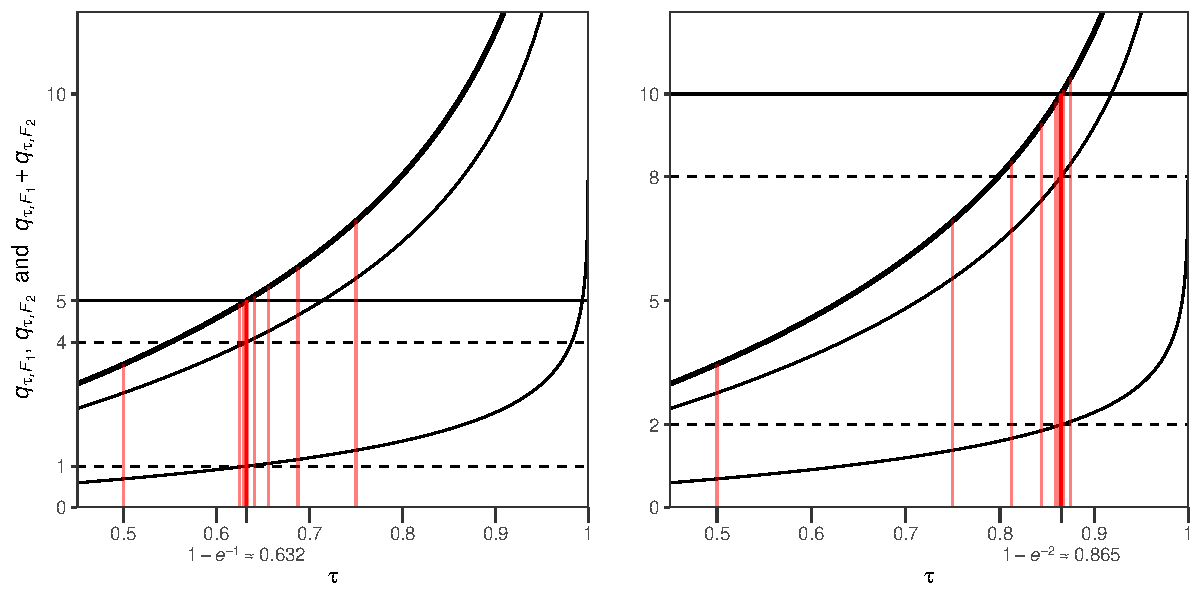
\includegraphics[width=\maxwidth]{figure/bisection-1} \caption{\DIFaddFL{Illustrations of bisection method for the examples of Section 2.1. In each plot the thinner black curves are the quantile functions of the exponential forecasts for Location 1, with $\sigma_1=1$ (lower), and Location 2, with $\sigma_2=4$ (upper), while the thicker black curve gives the sum of these quantiles, which must meet the resource constraints of $K = 5$ on the left and $K=10$ on the right. The red segments show the iterates $\tau_{M,j}$ and their associated total resource demands as given by the function }\texttt{\DIFaddFL{allocate}} \DIFaddFL{from the package }\texttt{\DIFaddFL{alloscore}} \DIFaddFL{applied to these examples and using an initial search interval $[0,1]$. (The $\tau_{M,j}$ are in this case just sums of terms $\pm 2^{-j}$.) The horizontal dashed lines show the resulting allocations (cf. Figure 1).}}\label{fig:bisection}
      \end{figure}

    \end{knitrout}

    \DIFaddend
  \end{mybox}

We also note that in order to refer to the closed form of the allocation levels for the examples of section 2.1 we numbered the relevant formula in 
Appendix section B:


\begin{mybox}{pg19-para4>>pg20-para1}
  An immediate consequence used in the examples in Section 2.1 is that if
  $F_i = \mathrm{Exp}(1/\sigma_i)$ for all $i$, then the Bayes act is proportional to $(\sigma_1,\ldots,\sigma_N)$, since
  \DIFdelbegin \DIFdel{$q_{\mathrm{Exp}(1/\sigma),\tau} = -\sigma \log(1-\tau)$.
  }\DIFdelend \DIFaddbegin \begin{align}
  \DIFadd{q_{\mathrm{Exp}(1/\sigma),\tau} = -\sigma \log(1-\tau). \tag{\color{blue}{\uwave{(14)}}}
}\end{align}
  \DIFaddend 
\end{mybox}


\begin{quotebar}
\begin{enumerate}
  \item[3.] The manuscript introduces the integrated allocation score (IAS) in Section 2.2.3. While the concept is well-founded, it does not describe the practical computation of this score. Have the authors developed any algorithms for these calculations? If so, it would be better to include a brief discussion.
\end{enumerate}
\end{quotebar}

We have not developed any special algorithms for the purpose of calculating the IAS, and see investigations as likely requiring 
the kind of \textit{ad hoc} approximation we use in (what is now) section 3.5.5.  To clarify this we have added text after our definition of the IAS:

\begin{mybox}{pg8-para2}
 However, if $K$ is not precisely known at the time of decision making or there is interest in measuring the
value of forecasts across a range of decision making scenarios with different resource constraints, we can use an
\emph{integrated allocation score} (IAS) that integrates the allocation score across values of $K$, weighting by a
distribution $p$:
\begin{equation}
S_{IAS}(F, y) = \int S_A(F,y; K) p(K) \, dK \tag{\color{blue}{\uwave{(8)}}} 
\end{equation} 
We note that the device of considering a range of hypothetical decision makers or decision making problems with
different problem parameters has been employed in the past (e.g., Murphy, 1993).

\DIFaddbegin \DIFadd{In practice, it may be challenging to compute the integral in (8).
In the applied investigations below we resort to a discretization, evaluating at a grid of values of the resource constraint $K$.
A discrete treatment along these lines will often be natural, in settings where the resource in question is non-divisible (e.g., ventilators, masks).
}
\DIFaddend 
\end{mybox}

We also added some clarifying text to section 3.5.5 to indicate how an approximation to the IAS was computed in our example:

\begin{mybox}{pg15-para2}
  \DIFaddbegin \subsubsection*{3.5.5 \quad \DIFadd{Integrated allocation score across values of K}}
  \label{sec:ias_examp}

  \DIFaddend The integrated allocation score (IAS) summarizes allocation scores (AS) across a range of possible values of the
  constraint ($K$), allowing one to assign higher weights to more likely values of $K$ (Section
 2.2.3). 
  IAS was computed for two weight distributions on \DIFaddbegin \DIFadd{the same grid of values of }\DIFaddend $K$ \DIFaddbegin \DIFadd{used in the sensitivity analysis above}\DIFaddend ,
  one uniform across the entire range and the other \DIFaddbegin \DIFadd{with weights proportional to }\DIFaddend a truncated normal distribution centered at 15,000
  (the orange and blue shaded areas in Figure
  6A, respectively).
  \DIFaddbegin \DIFadd{With these weight distributions, the IAS defined in Equation (8) can be computed as the sum
  }$$\DIFadd{S_{IAS}(F, y) = \sum_K S_A(F,y; K) p(K)}$$

  \DIFaddend 

\end{mybox}
We would expect such an approximation to be available and appropriate in general.

\begin{quotebar}
\begin{enumerate}
  \item[4.] The proposed AS rule focuses on addressing immediate resource needs like hospital admissions and static resources. While this focus is practically significant, it may be too simplistic to capture the complex, dynamic nature of public health management. The framework notably excludes preventative measures such as vaccines, which are crucial for reducing future disease incidence. It would be beneficial for the authors to discuss the challenges and potential method- ologies for incorporating these preventative aspects and dynamic resources into the scoring rule.
\end{enumerate}
\end{quotebar}

In order to be more transparent regarding the scope of this paper we have rewritten part of the discussion section to collect limitations mentioned earlier 
(such as those relating to vaccines in paragraph 2 of section 2.2.2) and give some brief methodological suggestions on how they could be confronted:


\begin{mybox}{pg17-para3>>pg17-para4}

  There are \DIFdelbegin \DIFdel{several }\DIFdelend \DIFaddbegin \DIFadd{three }\DIFaddend important limitations to the current work \DIFdelbegin \DIFdel{. The allocation score we developed here }\DIFdelend \DIFaddbegin \DIFadd{which we noted when introducing the AS in 
    Section 2.2.2.  We view these issues as promising avenues for 
    future investigation.
  }

  \DIFadd{First, the terms in our loss function  
    (3) do not depend on geographic or demographic covariates.  Policy makers may, however, wish to incorporate 
    differences in the impact of unmet need across populations into a forecast evaluation methodology.  For example, in the state-level forecasting context of Section 3, it might be
    appropriate to adjust the loss so that the costs of unmet need are larger in locations with greater population vulnerability.
  Along these lines, it should also be mentioned that the AS }\DIFaddend does not directly
  \DIFdelbegin \DIFdel{account for important considerations such as }\DIFdelend \DIFaddbegin \DIFadd{take into consideration the }\DIFaddend fairness or equity of allocations, or more broadly, individual and group
  preference relations that are difficult or even impossible to encode into a loss or utility function.  Ambiguity aversion
  (in the sense of Ellsberg (1961)), for example, seems especially relevant to the use of forecasts in outbreak
  response, where there can be immense social and political pressure on public health officials to maintain a transparent
  base of evidence for their policy choices and recommendations. 
  \DIFdelbegin \DIFdel{The proposed framework also does not attempt to capture
    the broader context of decision making. For example, in practice it may be possible to increase the resource constraint
  $K$ by shifting funding from other }\DIFdelend 

\DIFaddbegin \DIFadd{Secondly, our formulation of the AS does not take into consideration
the temporal 
inter-dependencies between sequential decisions that public
health decision makers are likely to face as an epidemic unfolds. Such
dependencies could arise from time-varying inputs such as resource
availability or the current effective allocations of resources. The
sequential decision problem could also be combined with others allowing
constraints for different resources to be modified by time-varying funding
shifts between various } \DIFaddend disease mitigation measures.  
\DIFdelbegin \DIFdel{Finally, } \DIFdelend 
\DIFaddbegin \DIFadd{Incorporating these
possibilities into an AS framework would likely require technical
developments involving either dynamic programming (see e.g., Bertsekas
(2012)) or a scenario-based approach (see e.g., Pflug and Pichler (2014)).}

\DIFadd{Thirdly, }\DIFaddend we emphasize that we opted at this stage of
development to explicitly rule out situations where a successful
epidemiological forecast could lead to policy decisions that change the
distribution of the predicted outcome $Y$. \DIFdelbegin \DIFdel{Our framework
would need considerable enhancements before being applicable }\DIFdelend
\DIFaddbegin \DIFadd{For example, this excludes the important problem of 
allocation of doses of a preventative vaccine. We have not developed a formal
approach }\DIFaddend to forecast evaluation \DIFdelbegin \DIFdel{beyond
horizons for which causal feedback can be neglected}\DIFdelend \DIFaddbegin
\DIFadd{using scores given by (7) when both disease burden and unmet need are
considered as endogenous variables. Such an approach would require some form
of accounting for the causal effect of the allocation decision on observed
measures of disease burden, e.g. using the available observed data to
estimate the (counterfactual) number of cases or deaths averted from one or
another allocation strategy}\DIFaddend.

\DIFdelbegin \DIFdel{An }\DIFdelend \DIFaddbegin \DIFadd{Another }\DIFaddend
opportunity for further investigation is to more carefully evaluate whether
forecasts add value to standard  procedures already in place for making public
health decisions. In the context of allocations, such a procedure might
extrapolate need from current observed need and population levels (similarly to
the two benchmark approaches presented above), with adjustments based on other
political or real-world considerations.
\end{mybox}


\begin{quotebar}
\begin{enumerate}
  \item[5.] The authors propose using unmet need as a loss function, which simplifies the model. However, this approach may not fully account for the diverse impacts of unmet needs across different locations and demographics. Could the authors explore the possibility of incorporating different weights or more complex loss functions to provide deeper insights, such as considering factors like population vulnerability.
\end{enumerate}
\end{quotebar}

We agree that the loss function we have formulated makes many simplifying assumptions, but we feel this simplification 
is necessary to keep the discussion in the paper of a manageable length.
Some of the complexities the referee mentions were noted in the manuscript section 2.2.2, where we first introduce the loss function:
“A variety of extensions are possible….”
However, we agree that these are important limitations of our initial formulation of the AS, 
and we have therefore added an additional mention of these possible extensions in the second paragraph of the changed text \textbf{pg17-para3>>pg17-para4} above
in the discussion section.


\begin{quotebar}
\begin{enumerate}
  \item[6.] To make the work more accessible to a general audience, it could be beneficial to establish connections with other fields such as economics, sociology, or urban planning. This could enrich the resource allocation framework presented in this paper, while also allow the findings to potentially benefit decision-making processes in those fields.
\end{enumerate}
\end{quotebar}

We have added several references to the end of the first paragraph in the discussion section, indicating other fields where decision making based on forecasts 
might benefit from the perspective we develop:


\begin{mybox}{pg16-para1}
\section*{4 \quad Discussion}
\label{sec:discussion}

Probabilistic forecasts of infectious disease outbreaks have typically been evaluated using well-known proper scoring
rules such as the LS, CRPS, and WIS. Often models are ranked according to such a score, but without reference to any
underlying decision problem from which the score might be derivable as a Bayes scoring rule or be otherwise motivated. 
We argue that the value of collaborative forecasting efforts, such as the COVID-19 Forecasting Hub, could be enhanced by
including evaluations of forecasts with
scoring rules that directly consider the success of forecasts in supporting specific \DIFdelbegin \DIFdel{public health decisions. As evidence for this possibility, we }\DIFdelend \DIFaddbegin \DIFadd{decisions.
The allocation score was developed for this purpose. The AS is expressed in units that are directly relevant to decisions, which helps not only with ranking forecasts in the context of a specific action, but also allows decision-makers to contextualize the magnitude of differences between forecast scores. For example, it may be the case that differences in AS are small relative to the amount of available resources or the accuracy with which planned resource allocations can be executed.
The benefits of the approach to forecast evaluation discussed here generalize beyond public health, to any application of probability forecasts for decision-making, such as economics, where the monetary consequences of using a forecast
can be clearly juxtaposed with standard accuracy measures of the forecast (Bannigidadmath and Narayan, 2016; Zhang et al., 2019), resource allocation in urban planning (Burnett, 2014; Liang and Wey, 2013), or sustainability initiatives such as water and energy allocation (Syme et al., 1999; Gebre et al., 2021; Colett et al., 2016).
}

\DIFadd{We }\DIFaddend have demonstrated how tying forecast evaluation to a specific decision problem (e.g., via the allocation
score) can yield model rankings that differ substantively from those based a current standard measure of forecast
accuracy, the WIS, which does not refer to any decision problem that has been clearly connected to outbreak response.
This result aligns with findings in other fields \DIFdelbegin \DIFdel{, especially those where the monetary consequences of using a forecast
can be clearly juxtaposed with standard accuracy measures of the forecast (Leitch and Tanner, 1991; Murphy, 1993; Cenesizoglu and Timmermann, 2012). }\DIFdelend Additionally, we show that an existing
ensemble forecast approach was the only method to outperform (in terms of this new evaluation method) two benchmark
allocation approaches in a hypothetical application, suggesting that there is room for innovation of current
epidemiological modeling techniques that might be spurred on by a reorientation of the field toward practical decision
problems. For example, in order to surpass benchmark allocation scores, forecasters need to devote effort to capturing
the \emph{relative} magnitude of future resource need across different locations.  Success at this task is not, however,
directly rewarded by the WIS \DIFaddbegin \DIFadd{(see the discussion at the end of Section (2.3))}\DIFaddend . 
\end{mybox}

We also sought a more general tone in our concluding paragraph by addressing it to decision-makers rather than just public health officials:

\begin{mybox}{pg18-para1>>pg18-para4}
New collaborative work between \DIFdelbegin \DIFdel{public health officials }\DIFdelend \DIFaddbegin \DIFadd{decision-makers }\DIFaddend and modeling teams is
needed to assess the value and relevance of the initial findings presented here, including real-time pilot studies or
simulation exercises that could be used to inform further development of new or alternative scoring metrics.
\end{mybox}

\section*{Comments from Referee 2}

\begin{quotebar}
Comments to the Author
Summary:
Gerding et al. advocate for new scoring rules for infectious disease forecasts that are explicitly based on resource allocation and other policy decision considerations. The authors consider a situation, where a forecaster produces multiple forecasts for different geographical locations that are under the jurisdiction of the same policy making agency (e.g., counties in a state or states/provinces/regions in a country). This is a reasonable setting that mimics policy decisions that had to be made during the COVID-10 pandemic and that are routinely being made during flu/COVID/RSV seasons. In particular, Gerding et al. develop their scoring rule using a decision theoretic framework with a loss function equal to the number of unmet need in bed allocations across all geographic areas under consideration. I think the manuscript is definitely a step in the right direction. It is really well written, with methods rigorously evaluated. Congrats on a great paper!


Paper strengths:

1. Evaluation of probabilistic infectious disease forecasts is an important area of research, so the authors' contribution to this area of research is timely.

2. The authors operate within a rigorous decision theoretic framework when deriving their score of the forecast skill and think deeply about policy decisions. 
\end{quotebar}

We thank the referee for the positive assessment of our work and highlighting feautures that we also feel make the larger research project worthwhile.

\begin{quotebar}
1. It is my understanding that currently most forecasts evaluated by the authors operate by producing forecasts independently across spatial locations. In other words, most forecasters do not produce joint probabilistic forecasts of all locations in the region of interest, for example using some complicated method that models all hospital beds in all graphic locations jointly. However, the score suggested by the authors explicitly evaluates these forecasts jointly. So my question is the following: is it possible that if the forecasts were produced jointly, the difference between WIS and AS would be less pronounced? Is it possible to illustrate this point on some toy forecasting problem? I think this could be important for stimulating development of multivariate forecasts across spatial locations -- a difficult problem computationally, but important to solve eventually for us as a community.
\end{quotebar}

We have tried to offer some initial clarification on the very important issue above in \textbf{author response 1}, but the referee's question is a broad one
and we feel that this paper is probably too confined a venue for us to do it justice. It does seem likely to us that if a forecaster tries to improve their forecast by introducing valid and identifiable inter-location dependency terms into their model, that this will tend to improve AS more than it improves WIS.  It also seems likely that the AS will be more effective than WIS at discriminating between forecasters using better or worse inter-location dependency specifications. 
But testing such conjectures is difficult since we cannot “control” for the marginal forecasts, and these are the only direct inputs that the AS sees.


\begin{quotebar}
2. One of the strengths of the new AS is its interpretability. I would like to encourage the authors to highlight this strengths more. One common complaint about WIS that I hear from applied epidemiologists and policy makers is that it is hard to understand what it means. The AS, if I understand it correctly, doesn't have this problem. This opens an opportunity for not only ranking forecasts but also identifying if they are meaningfully different from each other. For example, two forecasts with AS scores of 400 and 380 may not be considered meaningfully different from each other if the total number of available hospital beds was 15,000. A policy maker may have prior knowledge that says that in practice implementing bed allocations across multiple locations according to a forecast is possible only up to some percentage of the total number of beds available. So +/- 20 beds could be smaller than the number of beds that would be misallocated due to logistical problems, human errors, medical personnel illnesses, etc.
\end{quotebar}

We appreciate this encouragement and look forward to emphasizing the interpretability advantages of the AS in future applied work.  In order to draw 
a bit more attention this strength we have rephrased the third paragraph of the introduction:

\begin{mybox}{pg2-para2}
While \DIFdelbegin \DIFdel{it should be noted that there are ways to interpret }\DIFdelend any of these scores \DIFdelbegin \DIFdel{abstractly }\DIFdelend \DIFaddbegin \DIFadd{can be interpreted }\DIFaddend through the lens of decision theory, \DIFdelbegin \DIFdel{and that all of the application-specific papers cited above benefited from direct collaboration with public
health agencies, a key impetus for the present work has been that we were not able to find in any of them, nor in the
literature they represent, }\DIFdelend \DIFaddbegin \DIFadd{they lack }\DIFaddend explicit connections between how a forecast \DIFdelbegin \DIFdel{was }\DIFdelend \DIFaddbegin \DIFadd{is }\DIFaddend evaluated and how that forecast was used in practice. \DIFaddbegin \DIFadd{A key impetus for the present work was to develop a score that is interpretable to decision makers by measuring the extent to which forecasts lead to improved decisions. In addition, the allocation score we propose is expressed in units that are intelligible to decision makers.
}\DIFaddend 
\end{mybox}

The ability that the AS gives decision-makers to contextualize differences in forecaster scores is also now mention in the first paragraph of the
Discussion section -- see change \textbf{pg16-para1} above.

\end{document}
